\documentclass[a4paper]{article}

\usepackage[UTF8]{ctex}
\usepackage[a4paper,margin=1in]{geometry}
\usepackage{graphicx}
\usepackage{float}
\usepackage{listings}
\usepackage{booktabs}
\usepackage{color}
\usepackage{indentfirst}
\setlength{\parindent}{2em}
\usepackage{zhnumber}
\usepackage{adjustbox}
\usepackage{subcaption}
\usepackage{amsmath}
\usepackage{amssymb}
\usepackage{enumitem}
\usepackage{lmodern}
\usepackage{inconsolata}
\usepackage{multirow}
\usepackage{tikz}
\usetikzlibrary{positioning}
\usepackage{fancyhdr}
\usepackage{hyperref}

% 配置lstlisting支持中文
\lstset{
    language=C,
    basicstyle=\footnotesize\ttfamily,
    breaklines=true,
    keywordstyle=\bfseries\color{blue},
    commentstyle=\itshape\color{green!50!black},
    stringstyle=\bfseries\color{red},
    numbers=left,
    numberstyle=\tiny\color{gray},
    frame=single,
    backgroundcolor=\color{gray!5},
    showstringspaces=false,
    keepspaces=true,
    tabsize=4,
    extendedchars=true,
    inputencoding=utf8,
    literate={，}{{\textcolor{green!50!black}{，}}}{1}
             {。}{{\textcolor{green!50!black}{。}}}{1}
             {：}{{\textcolor{green!50!black}{：}}}{1}
             {；}{{\textcolor{green!50!black}{；}}}{1}
             {（}{{\textcolor{green!50!black}{（}}}{1}
             {）}{{\textcolor{green!50!black}{）}}}{1}
             {【}{{\textcolor{green!50!black}{【}}}{1}
             {】}{{\textcolor{green!50!black}{】}}}{1}
}

\newcommand{\projname}{计算机网络实验|实验四}
\newcommand{\reporttitle}{访问控制个人心得体会}
\newcommand{\groupno}{第一组}
\newcommand{\authorname}{马福泉}
\newcommand{\major}{计算机科学与技术}
\newcommand{\adviser}{谢逸}
\newcommand{\startdate}{2025年10月27日}
\newcommand{\labenddate}{2025年11月5日}
\newcommand{\labroom}{实验D402}

\pagestyle{fancy}
\fancyhf{}
\fancyhead[L]{\kaishu \projname}
\fancyhead[C]{\kaishu \reporttitle}
\fancyhead[R]{\kaishu \authorname}
\fancyfoot[C]{第 \thepage 页}
\renewcommand{\headrulewidth}{0.4pt}
\renewcommand{\footrulewidth}{0pt}


\begin{document}

% 封面
\begin{titlepage}
    \centering
    
\includegraphics[width=10cm]{img/SYSULogo.png}
    \vspace{1em}
    % 修改为换行并居中
    \par
    {\Large \kaishu
        \par
        \projname
        \par
    }
    \vspace{3em}
    {\fontsize{40pt}{42pt}\kaishu \selectfont \boldmath \reporttitle\par}
    \vspace*{\fill}
    \begin{center}
    {\Large
    \makebox[5em][s]{姓名}:\underline{\makebox[15em][c]{\kaishu 马福泉}}\\[1em]
    \makebox[5em][s]{学号}:\underline{\makebox[15em][c]{\kaishu 23336179}}\\[1em]
    \makebox[5em][s]{小组编号}:\underline{\makebox[15em][c]{\kaishu \groupno}}\\[1em]
    \makebox[5em][s]{专业}:\underline{\makebox[15em][c]{\kaishu \major}}\\[1em]
    \makebox[5em][s]{课程教师}:\underline{\makebox[15em][c]{\kaishu \adviser}}\\[1em]
    \makebox[5em][s]{起始日期}:\underline{\makebox[15em][c]{\kaishu \startdate}}\\[1em]
    \makebox[5em][s]{结束日期}:\underline{\makebox[15em][c]{\kaishu \labenddate}}\\[1em]
    \makebox[5em][s]{实验地点}:\underline{\makebox[15em][c]{\kaishu \labroom}}
    }
    \end{center}
    \vspace*{\fill}
\end{titlepage}

\section{承担的工作}

\subsection{主要工作}
\begin{itemize}
    \item 负责协助进行实验设备的连接，包括PC与路由器的物理连接，根据队友重新绘制的拓扑图连接网线并验证连接状态
    \item 配置PC的IP地址、子网掩码和默认网关等网络配置
    \item 辅助队友参与R1和R2的GigabitEthernet接口IP地址配置和接口激活工作
    \item 参与标准ACL（实验8-1）的配置与测试，协助完成ACL 2025的创建和应用，验证PC2无法访问PC3而PC1可以访问的实验要求
    \item 参与高级ACL（实验8-2）的配置工作，协助完成ACL 3001的创建，实现基于端口号和IP地址的精细化访问控制
    \item 辅助队友搭建FTP和WWW服务器，协助配置Windows IIS服务、防火墙设置、文件夹权限设置等工作
    \item 参与实验验证和抓包分析工作，使用Wireshark抓取并分析FTP和HTTP协议的数据包
\end{itemize}

\section{遇到的困难及解决方法}

\subsection{硬件设备相关问题}
\begin{itemize}
    \item \textbf{端口不可用问题：}实验手册指明的路由器4、5接口实际上不可用，导致无法按原计划连接设备。通过队友重新绘制拓扑图，我们将接口改为0/0/0和0/0/3等可用接口，并据此重新进行物理连接。
    \item \textbf{端口识别困难：}路由器端口编号不连续，容易连接错误，以前就试过这种情况，需要在连接后观察端口指示灯状态，确保物理连接的正确性。
\end{itemize}

\subsection{ACL配置相关问题}
\begin{itemize}
    \item \textbf{ACL编号冲突：}实验要求使用ACL 2001，但该编号已被设置为acl-basic-ssh-kongzhi，无法修改或使用。通过改用ACL 2025完成实验8-1的要求。
    \item \textbf{命令格式错误：}实验手册提供的ACL配置命令在实际设备上报"too many parameters"错误。这是本次实验卡住最关键的问题，花费了不少时间，最终通过查询华为官方技术文档，了解到AR6140E-9G-2AC型号路由器的正确命令格式，发现需要使用高级ACL（3000-3999）而非基本ACL（2000-2999），并按照正确的参数顺序重新配置。
\end{itemize}

\subsection{服务器搭建相关问题}
\begin{itemize}
    \item \textbf{第三方软件配置复杂：}最初尝试使用Filezilla Server和Apache Server搭建服务，但教程繁琐且容易出错。虽然Apache Server能够成功启动并监听80端口，但仍然无法从客户端访问。
    
    \begin{figure}[H]
        \centering
        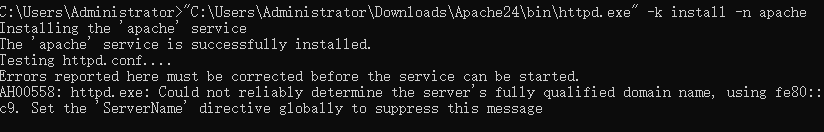
\includegraphics[width=0.8\textwidth]{img/apache1.png}
        \caption{Apache Server启动成功}
    \end{figure}
    
    \begin{figure}[H]
        \centering
        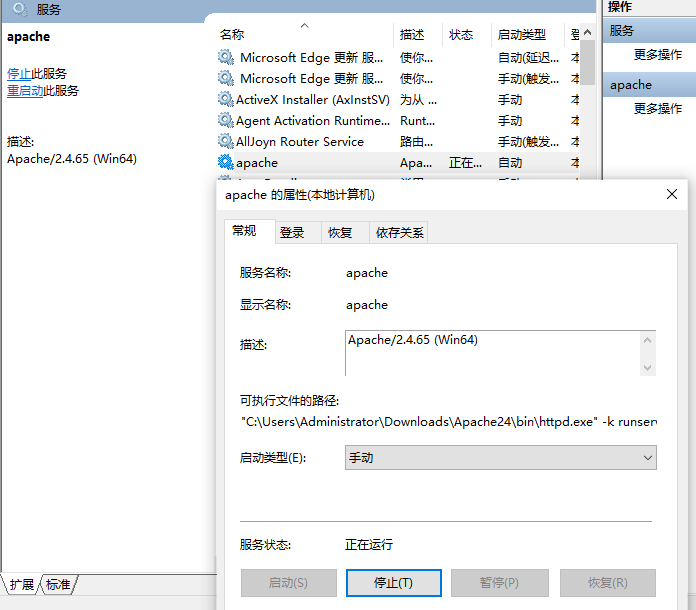
\includegraphics[width=0.8\textwidth]{img/apache2.png}
        \caption{Apache成功启用}
    \end{figure}
    
    经过分析，Apache Server配置成功但无法访问可能有以下几个原因：
    \begin{enumerate}[label=(\arabic*)]
        \item \textbf{Windows防火墙阻止：}Windows防火墙可能没有为Apache添加入站规则，即使端口80已监听，外部请求仍被阻止；
        \item \textbf{IIS与Apache端口冲突：}可能是因为原来的PC已经安装了IIS，如果系统同时安装了IIS和Apache，两者都默认使用80端口，可能导致Apache虽然启动但实际无法正常监听；
        \item \textbf{httpd.conf配置问题：}我查阅相关博客，对Apache的主配置文件中的许多文件进行了配置和修改，但是可能存在相关配置错误，导致无法正常响应请求；
    \end{enumerate}
    
    由于排查Apache配置问题较为耗时，最终改为使用Windows自带的IIS服务，简化了配置流程并成功搭建了WWW服务器。
    \item \textbf{服务无法访问：}FTP和WWW服务配置完成后无法从客户端访问。经排查发现是防火墙阻止了连接，通过在防火墙中允许所有与FTP、WWW相关的入站和出站连接解决问题。
    \item \textbf{文件夹权限问题：}服务仍然无法访问，进一步排查发现物理路径文件夹为只读且权限不足。通过去除只读属性、给予所有用户完全控制权限、设置文件夹共享，最终解决了访问问题。
    \item \textbf{多IP地址配置：}PC3需要同时提供FTP和WWW服务，需要配置两个IP地址以便区分。通过在网络适配器的高级设置中新增IP地址192.168.4.3作为WWW服务器地址，192.168.4.22作为FTP服务器地址。
\end{itemize}

\subsection{理论理解相关问题}
\begin{itemize}
    \item \textbf{ACL匹配顺序：}对ACL规则的匹配机制理解不够深入。通过学习了解到ACL规则从上到下逐条匹配，找到第一条匹配规则后即执行相应动作，所有规则都不匹配时默认拒绝。
    \item \textbf{FTP协议工作流程：}对FTP的控制连接和数据连接机制不够清楚。通过抓包分析，理解了FTP使用21端口建立控制连接，20端口进行数据传输，以及主动模式和被动模式的区别。
    \item \textbf{基本ACL与高级ACL的区别：}对两种ACL的功能差异认识不足。通过查阅文档和实验验证，理解了基本ACL只能基于源IP地址过滤，而高级ACL可以同时基于源/目的IP地址、协议类型、端口号等多种条件进行精细化控制。
\end{itemize}

\section{体会与总结}
\subsection{技术收获}
\begin{itemize}
    \item \textbf{ACL原理掌握：}理解了ACL的工作原理，包括标准ACL和高级ACL的区别、匹配顺序（config/auto）、隐式拒绝规则、入站出站方向的选择等核心概念。
    \item \textbf{服务器搭建能力：}了解了使用Windows IIS搭建FTP和WWW服务器的基本步骤，掌握了防火墙配置、文件夹权限设置、服务端口配置等服务器部署的基本知识。
    \item \textbf{协议分析能力：}通过Wireshark抓包分析，加深了对TCP、FTP、HTTP等协议的理解，能够从数据包层面分析网络通信过程和问题原因。
    \item \textbf{故障排查方法：}掌握了系统性的网络问题排查方法，从物理层连接、网络层配置、传输层端口、应用层服务的逐层分析思路，以及利用ping、telnet、抓包等工具进行故障定位。
    \item \textbf{文档查阅能力：}提高了查阅官方技术文档的能力，能够快速定位问题并找到正确的解决方案，了解了华为ACL技术支持文档的结构和使用方法。
\end{itemize}

\subsection{实验体会}
\begin{itemize}
    \item 实践操作让我认识到网络安全配置中细节的重要性，ACL规则的顺序、方向、参数格式等任何一个细节错误都可能导致安全策略失效，培养了严谨细致的工作态度。
    \item 遇到问题时查阅官方技术文档的经验，让我认识到阅读原厂文档的重要性，不同设备型号的命令格式可能存在差异，需要以官方文档为准。
    \item 团队协作中的分工合作和问题讨论，提高了沟通协调能力和问题解决能力。
\end{itemize}
\end{document}
